\section{\itshape Data Streams  \textnormal{(Fluxos de  dados)}}

\begin{frame}{\textit{Data Streams}}
    \begin{columns}
	    \column{0.5\textwidth}\centering
	        Características de \textit{data streams}\footnotemark:
        	\begin{itemize}
        	    \item As amostras são obtidas continuamente, obedecendo uma determinada taxa de amostragem.
                \item O conjunto de dados é teoricamente ilimitado. 
                \item O processo de geração das amostras pode ser não estacionário.
        	\end{itemize}
        	
	    \column{0.5\textwidth}\centering
        	\begin{figure}
        	    \centering
        	    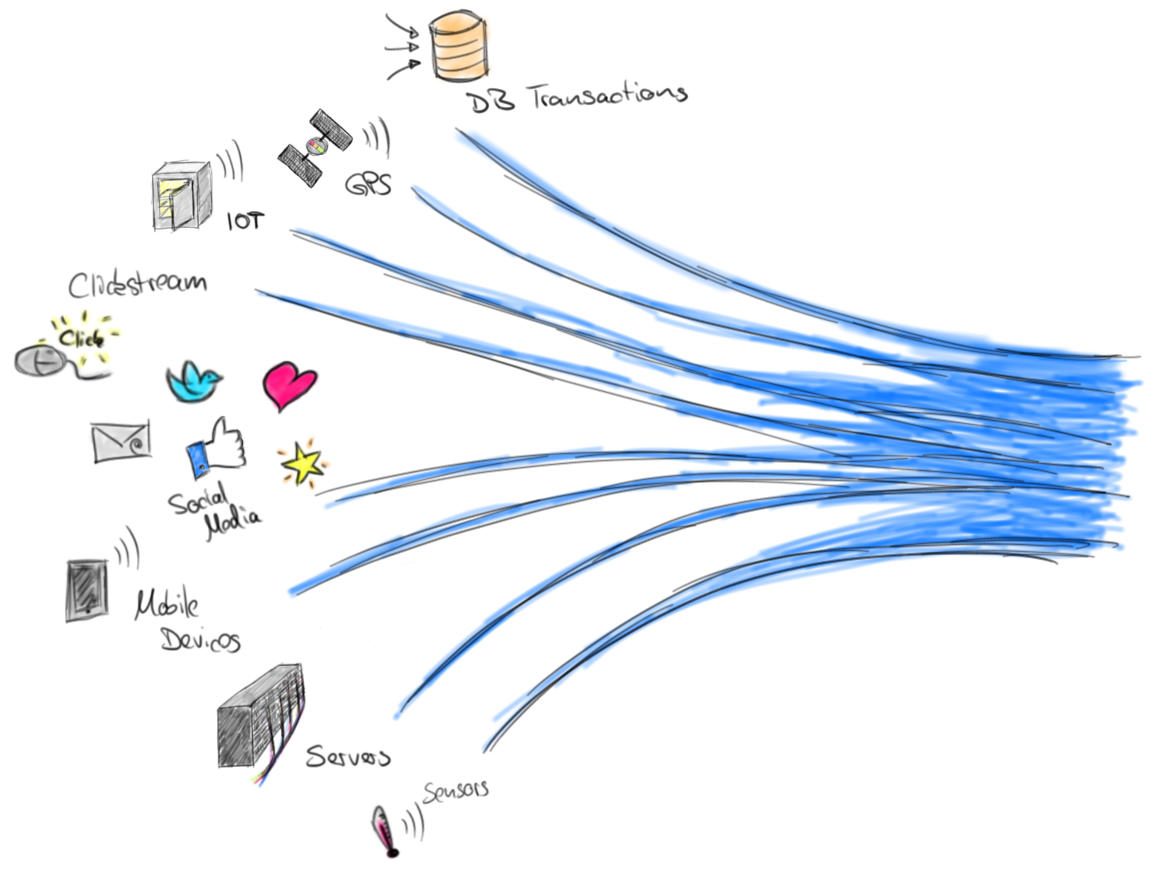
\includegraphics[width=\textwidth,height=\textheight,keepaspectratio]{figuras/streams.png}
        	    \caption{Ilustração de fluxos de dados}
        	    \label{fig:ilustracao_fluxo_dados}
        	\end{figure}
	\end{columns}
	\footnotetext{\cite{silva2013data}}
\end{frame}

\begin{frame}{\textit{Data Streams}}
	\begin{columns}
	    \column{0.5\textwidth}\centering
	        \textit{Concept Drift}
	        \begin{figure}
        	    \centering
        	    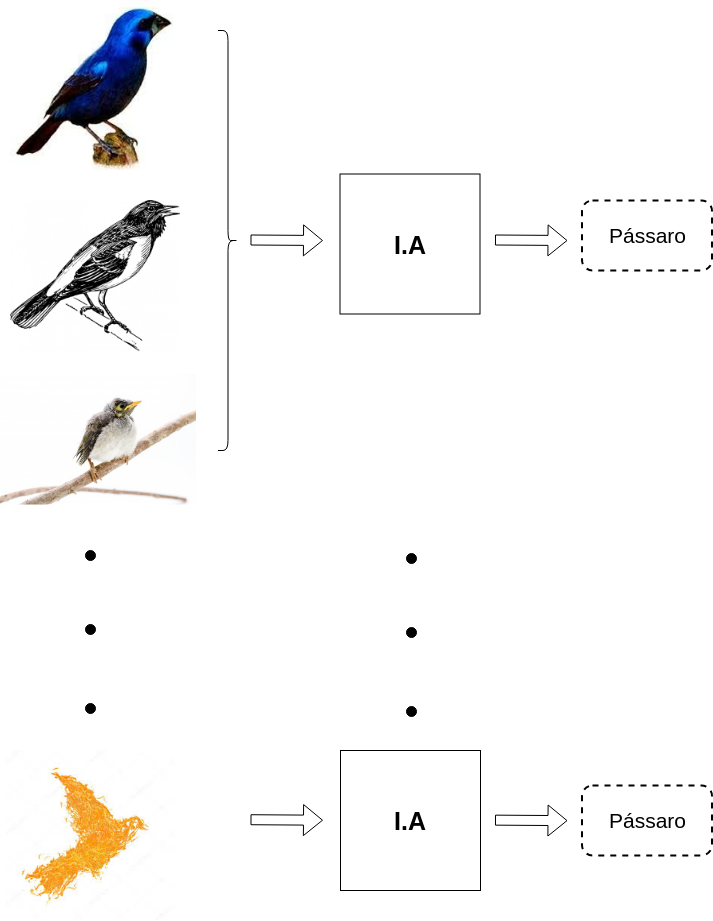
\includegraphics[height=.55\textheight,width=\textwidth,keepaspectratio]{figuras/passaros_brancas.png}
        	    \caption{Ilustração de \textit{concept drift}}
        	    \label{fig:concept_drift}
        	\end{figure}
	        
	    \column{0.5\textwidth}\centering
	        \textit{Concept Evolution}
	        \begin{figure}
        	    \centering
        	    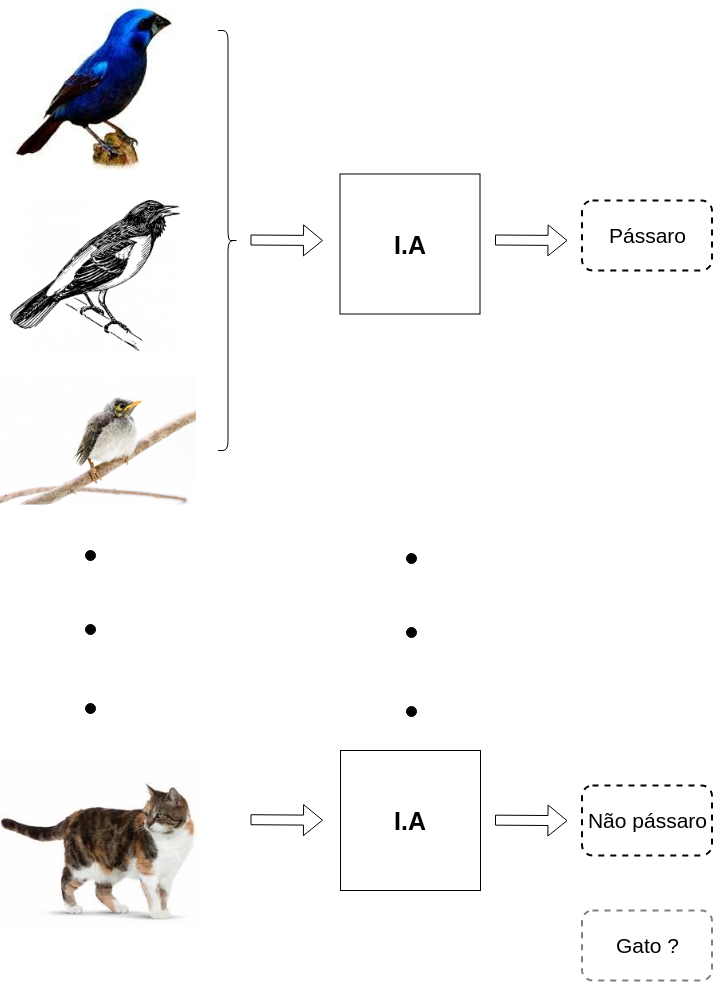
\includegraphics[width=\textwidth,height=.55\textheight,keepaspectratio]{figuras/passaros_gatos.png}
        	    \caption{Ilustração de \textit{concept evolution}}
        	    \label{fig:concept_evolution}
        	\end{figure}
	\end{columns}
\end{frame}


\begin{frame}{Técnicas de Processamento de \textit{Data Streams}}
	\begin{itemize}
	    \item RDE\footnote{\cite{angelov2012autonomous}}: Algoritmo para cáculo recursivo da densidade de \textit{data streams} para finalidade de detecção de \textit{outliers}.
	    \item TEDA\footnote{\cite{angelov2014anomaly}}: Algoritmo para detecção de \textit{outliers} baseado em \textbf{tipicidade} e \textbf{excetricidade}
	    \item AutoCloud\footnote{\cite{bezerra2017abordagem}}: Algoritmo para clusterização de \textit{data streams} baseado no TEDA.
	\end{itemize}
	\pause

	Técnicas para processamento de \textit{data streams} necessitam ligar com \textit{concept drift} e \textit{concept evolution} além operar de maneira recursiva nos novos dados da \textit{stream}
\end{frame}